%%%%%%%%%%%%%%%%%%%%%%%%%%%%%%%%%%%%%%%%%%%%%%%%%%%%%%%%%%%%
\section[Bilder, Grafiken und Diagramme]{Bilder, Grafiken und Diagramme}
\label{sec:Bilder}
%%%%%%%%%%%%%%%%%%%%%%%%%%%%%%%%%%%%%%%%%%%%%%%%%%%%%%%%%%%%
%
Bei Einbindung von Grafiken sind zwei Fälle zu unterscheiden:
\begin{itemize*}
  \item reguläre \index{Bild!Binär-}Bilder in einem Binärformat
	      (\texttt{PNG}, \texttt{TIFF}, \texttt{JPG}, \texttt{PDF}, etc.)
	\item \index{Bild!Vektor-}Grafiken, die im \gls{gls:tikz}-Quellcode vorliegen 
\end{itemize*}

Grundlegender Unterschied bei der Einbindung \enquote{regulärer} Bilder
und \gls{gls:tikz}-Bilder ist, dass Binärformatgrafiken mit \lc{includegraphics\{...\}}
eingebunden werden, während \gls{gls:tikz}-Grafiken mit \lc{input\{...\}} eingebunden
und von \texttt{latex} mitkompiliert werden.


%%%%%%%%%%%%%%%%%%%%%%%%%%%%%%%%%%%%%%%%%%%%%%%%%%%%%%%%%%%%
\subsection[Floats]{\index{Float}\index{Bild!Float}Floats}%
\label{sec:Floats}
%%%%%%%%%%%%%%%%%%%%%%%%%%%%%%%%%%%%%%%%%%%%%%%%%%%%%%%%%%%%
%
Üblicherweise werden Bilder und Tabellen in Fließumgebungen (floats) gesetzt,
damit \LaTeX\ sie geschickt positionieren kann.
Bei Bildern heißt die entsprechende Float-Umgebung \printkeyword{figure}.
Die Positionierung kann durch Angabe von Buchstaben
\printkeyword{h}, \printkeyword{t}, \printkeyword{b} und \printkeyword{p}
beeinflusst werden
(\enquote{here}, \enquote{top}, \enquote{bottom}, \enquote{extra page}).

\myexcl{Wichtig!}
Seitens des \glsgen{ac:KSP} wird bezüglich Einbindung von Floats gefordert,
dass diese die einzelnen Sätze nicht zerreißen.
Dies bedeutet, dass eine Platzierung von Bildern und Tabellen lediglich
zwischen zwei Absätzen in Frage kommt.
Allerdings kann es passieren, dass der Platz auf der Seite nicht mehr ausreicht,
und das Bild nicht an der gewünschten Stelle gesetzt werden kann.
Damit wird das Bild auf die nächste Seite verschoben.
Bei aktivierter \printkeyword{t}- oder \printkeyword{b}-Option würde \LaTeX{} versuchen,
das Bild am oberen oder unteren Rand der Seite zu platzieren.
Allerdings passiert das dann häufig mitten in einem Satz,
was vom \gls{ac:KSP} ausdrücklich nicht erwünscht ist.
Somit bleibt eigentlich nur noch die Verwendung der \printkeyword{h}-Option.

Leider können dabei einige unerwünschte Effekte auftreten.
So können beispielsweise auf der vorherigen Seite riesige leere Flächen entstehen.
Wenn der verbleibende Platz auf der Seite eine Platzierung nicht erlaubt,
kann es schnell passieren, dass \LaTeX{} das betroffene Bild 
und alle Folgeilder ans Ende des Kapitels verschiebt
(genauer gesagt, an die Stelle, wo die nächste \lc{clearpage}-Anweisung kommt).

Eine genaue Auswirkung der Parameter
\printkeyword{h}, \printkeyword{t}, \printkeyword{b} und \printkeyword{p}
auf die Bildplatzierung ist nicht immer intuitiv.
Um diese zu verstehen, empfiehlt sich die Lektüre der Beschreibung
von Frank Mittelbach
\href{https://tex.stackexchange.com/questions/39017/how-to-influence-the-position-of-float-environments-like-figure-and-table-in-lat/39020#39020}{auf stackexchange.com}.%
\footnote{\url{https://tex.stackexchange.com/questions/39017/how-to-influence-the-position-of-float-environments-like-figure-and-table-in-lat/39020#39020}}

Prinzipiell empfiehlt sich eine endgültige Platzierung der Bilder erst ganz am Schluss,
nachdem alle anderen Korrekturen durchgeführt sind.
Ggf. müssen die Bilderdefinitionen manuell im Quellcode herumgeschoben werden,
bis die Abbildungen von \LaTeX\ optimal gesetzt werden.
Dafür empfiehlt es sich, die einzelnen Bilddefinitionen in Extra-Dateien auszulagern,
so dass nur noch eine einzige Zeile herumgeschoben werden muss.

%%%%%%%%%%%%%%%%%%%%%%%%%%%%%%%%%%%%%%%%%%%%%%%%%%%%%%%%%%%%
\subsection[Binärbilder]{\index{Bild!Binär-}Binärbilder}%
\label{sec:Binaerbilder}
%%%%%%%%%%%%%%%%%%%%%%%%%%%%%%%%%%%%%%%%%%%%%%%%%%%%%%%%%%%%
%
Ein Beispiel für die Einbindung eines Bildes im Binärformat ist in \cref{lst:binary-image} angeführt:

\begin{latex}[caption={Einbindung einer Binärgrafik in LaTeX},label={lst:binary-image}]
\begin{figure}[h]%
  \centering%
  \includegraphics[width=\linewidth]{Bildpfad/Dateiname}%
  \caption[Kurzversion für das Abbildungsverzeichnis]{%
           Eine tolle sehr lange Abbildungsunterschrift}%
  \label{fig:my-binary-image}%
\end{figure}
\end{latex}

Die Angabe des Pfades kann sowohl absolut als auch relativ
zum Verzeichnis der Hauptdatei oder zu einem der Pfade angegeben werden,
die in der Datei \printfilepath{./preambel/AllePfade.tex} definiert sind.
Diese Pfade werden in angegebenen Reihenfolge durchsucht.
Dasselbe gilt für die Dateierweiterung.
Ist keine Erweiterung definiert und liegen mehrere Bilder mit gleichem Namen jedoch unterschiedlicher Dateierweiterung vor,
wird die Reihenfolge, die in der Datei texttt{AllePfade.tex} definiert ist, verwendet.

Zu beachten ist dabei, dass der \gls{ac:KSP} Skalierung der Bildern auf die Seitenbreite fordert,
was hier durch die Option \printkeyword{width=\bs linewidth} verwirklicht wurde.

Wichtig anzumerken ist, dass alle Zeilen innerhalb der \printkeyword{Figure}"=Umgebung
mit einem Prozentzeichen abzuschließen sind.
Ansonsten werden überflüssige Leerzeichen eingefügt,
was zu unerwünschten Nebenwirkungen führen kann.

Mit Hilfe von Paket \pkg{subfig} \cite{Cochran2005} können Bilder auch in
\index{Abbildung|see{Bild}}\index{Bild!Unterabbildung}Unterabbildungen gesetzt
und sowohl als ganzes (vgl. \cref{fig:subfloat-example}) als auch einzeln (vgl.
\cref{fig:subfloat-example-01,fig:subfloat-example-02,fig:subfloat-example-03,fig:subfloat-example-04})
referenziert werden.

\begin{figure}[h]%
	\centering%
	\subfloat[La Savoureuse, Lepuix, Frankreich (\copyright\ Thomas Bresson)]{%
		\label{fig:subfloat-example-01}%
		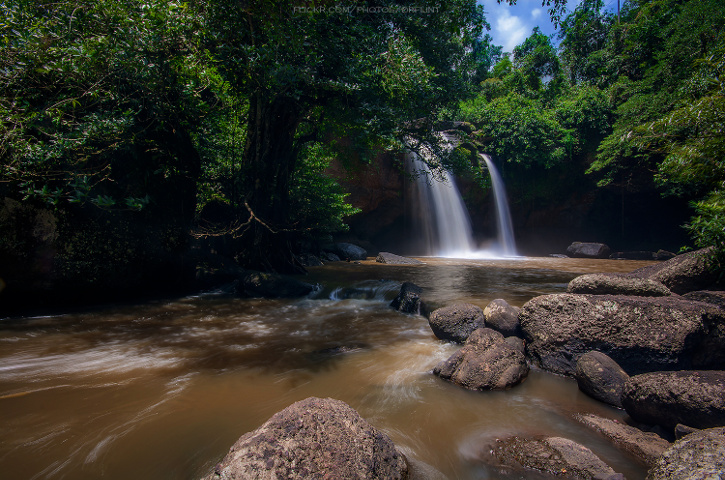
\includegraphics[width=0.49\linewidth]{./images/examples/subfloat-example-01.jpg}%
	}%
	\hfill%
	\subfloat[Bangkok, Thailand (\copyright\ Prachanart Viriyaraks)]{%
		\label{fig:subfloat-example-02}%
		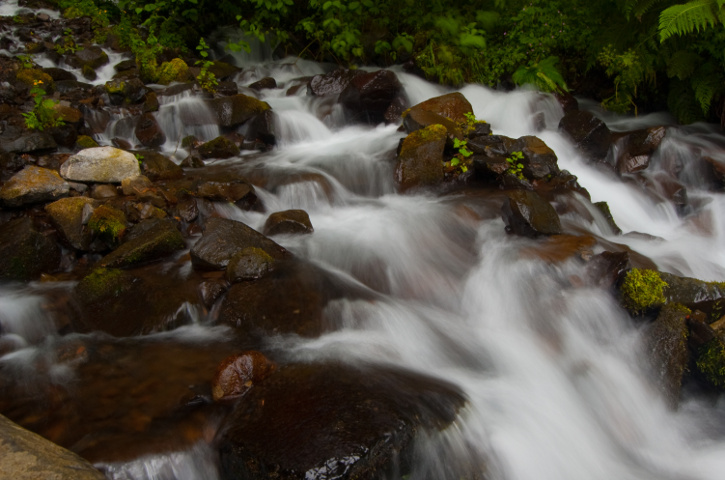
\includegraphics[width=0.49\linewidth]{./images/examples/subfloat-example-02.jpg}%
	}%
	\\%
	\subfloat[Wahkeena Falls, Lincoln Park, USA (\copyright\ srslyguys)]{%
		\label{fig:subfloat-example-03}%
		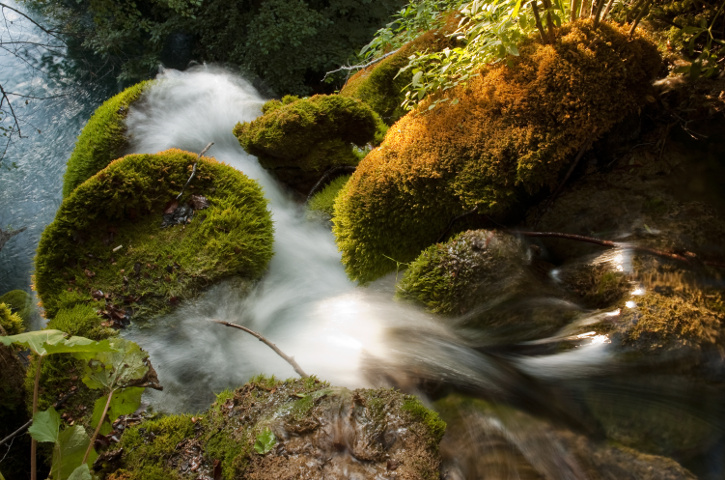
\includegraphics[width=0.49\linewidth]{./images/examples/subfloat-example-03.jpg}%
	}%
	\hfill%
	\subfloat[Nacionalni park Plitvička jezer, Kroatien (\copyright\ Roman Bonnefoy)]{%
		\label{fig:subfloat-example-04}%
		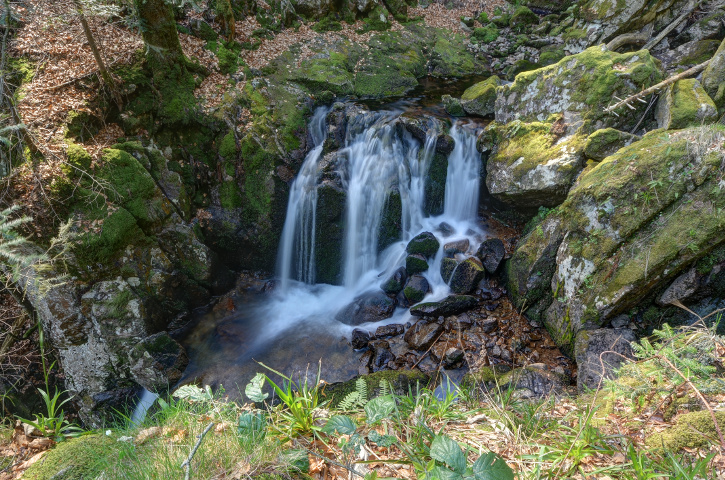
\includegraphics[width=0.49\linewidth]{./images/examples/subfloat-example-04.jpg}%
	}%
	\caption[Bild mit Unterabbildungen]{Wasserfälle der Welt als Beispiel für Unterabbildungen}%
	\label{fig:subfloat-example}%
\end{figure}

Der Beispielcode dafür ist in \cref{lst:subfigures} dargestellt.

\begin{latex}[caption={Unterabbildungen in LaTeX},label={lst:subfigures}]
\begin{figure}[h]%
	\centering%
	\subfloat[Unterbezeichnung 1)]{%
		\label{fig:UnterAbb1}%
		\includegraphics[width=0.49\linewidth]{Bildpfad/Bild1}%
	}%
	\hfill%
	\subfloat[Unterbezeichnung 2]{%
		\label{fig:UnterAbb2}%
		\includegraphics[width=0.49\linewidth]{Bildpfad/Bild2}%
	}%
	\\%
	\subfloat[Unterbezeichnung 3)]{%
		\label{fig:UnterAbb3}%
		\includegraphics[width=0.49\linewidth]{Bildpfad/Bild3}%
	}%
	\hfill%
	\subfloat[Unterbezeichnung 4]{%
		\label{UnterAbb4}%
		\includegraphics[width=0.49\linewidth]{Bildpfad/Bild4}%
	}%
\caption[Kurzversion]{Langversion der Bildunterschrift}%
\label{fig:MeinGanzesBild}%
\end{figure}
\end{latex}

Man beachte die abschließenden Prozent-Zeichen am Ende jeder Zeile!

%%%%%%%%%%%%%%%%%%%%%%%%%%%%%%%%%%%%%%%%%%%%%%%%%%%%%%%%%%%%
\subsection[TikZ-Grafiken]{\index{TikZ}\index{Bild!TikZ}\gls{gls:tikz}-Grafiken}%
\label{sec:TikZ}
%%%%%%%%%%%%%%%%%%%%%%%%%%%%%%%%%%%%%%%%%%%%%%%%%%%%%%%%%%%%
%
\Gls{gls:tikz} eignet sich hervorragend, um wissenschaftliche Zeichnungen,
Vektorgrafiken und \index{Diagramm}Diagramme direkt mithilfe von LaTeX
zu setzen, sodass die Schrift direkt zum restlichen Dokument passt.
Zu dem \pkg{tikz}-\gls{gls:pkg} und dem darauf aufsetzenden \pkg{PGFplots}-\gls{gls:pkg} gibt
es hervorragende Dokumentation \parencites{Tantau2013}{Feuersaenger2014}.
Mit \gls{gls:tikz} und \gls{gls:pgfplots} lassen sich viele gute Sachen machen.


Der Code für die Einbindung einer \gls{gls:tikz}-Grafik sieht folgendermaßen aus:
\begin{latex}[caption={Einbindung einer TikZ-Zeichnung in LaTeX},label={lst:tikz-figure}]
\begin{figure}[h]%
  \centering%
  \tikzsetnextfilename{TikZ-Bild}%
  \resizebox{\textwidth}{!}{%   <--- optionale Skalierung
    \input{./figures-src/TikZ-Bild.tex}%
  }%                            <--- optionale Skalierung
  \caption[Kurzversion für das Abbildungsverzeichnis]{%
           Eine tolle sehr lange Abbildungsunterschrift}%
  \label{fig:my-tikz-figure}%
\end{figure}
\end{latex}

Eine Skalierung auf die volle Seitenbreite oder ein vielfaches davon im Falle von Unterabbildungen kann bei Bedarf mit Hilfe der Anweisung
\texttt{\bs resizebox\{\bs textwidth\}\{!\}\{...\}}
durchgeführt werden.

Das Kommando \verb+\tikzsetnextfilename{...}+ ist nicht unbedingt notwendig,
 aber sehr zu empfehlen, da dies als Name für das temporäre Kompilat im Ordner
\printfilepath{./figures-compiled/} genommen wird.
Dieser sollte gleich dem Namen des Quelldatei (ohne Endung) gewählt werden.
Ansonsten nimmt \texttt{pdflatex} eine hochlaufende Nummer als Dateiname,
was die Fehlersuche sehr erschwert.

Nachfolgend finden sich einige Beispiele für TikZ-Zeichnungen, nämlich
eine Übersicht über die KIT-Corporate-Identity-Farben (\cref{fig:kit-colors}),
ein kommutatives Diagramm (\cref{fig:kpca}),
ein Netzwerkkommunikationsgraph (\cref{fig:net-comm}),
einfache \index{Diagramm!Punkt-}Punktdiagramme (\cref{fig:ica})
und etwas aufwendigere Diagramme mit mehreren
\index{Achsensystem|see{Diagramm}}Achsensystemen (\cref{fig:pca}).

\begin{figure}[hp]%
	\centering%
  \tikzsetnextfilename{kit-colors}%
	%\resizebox{\textwidth}{!}{%
		\begin{tikzpicture}[
box/.append style={rectangle,inner sep=0pt,outer sep=0pt,minimum size=1.5em,draw=none,fill=#1},
label/.style={font={\ttfamily\footnotesize},anchor=east},
caption/.style={font={\ttfamily\footnotesize},rotate=90,anchor=west}
]
\matrix[row sep=.2em,column sep=.2em] {
  &
\node[caption] {\textbackslash{}KITgreen...};      &
\node[caption] {\textbackslash{}KITblue...};       &
\node[caption] {\textbackslash{}KITblack...};      &
\node[caption] {\textbackslash{}KITpalegreen...};  &
\node[caption] {\textbackslash{}KITyellow...};     &
\node[caption] {\textbackslash{}KITorange...};     &
\node[caption] {\textbackslash{}KITbrown...};      &
\node[caption] {\textbackslash{}KITred...};        &
\node[caption] {\textbackslash{}KITlilac...};      &
\node[caption] {\textbackslash{}KITcyanblue...};   \\
\node[label] {};               &
\node[box=KITgreen      ] {};  &
\node[box=KITblue       ] {};  &
\node[box=KITblack      ] {};  &
\node[box=KITpalegreen  ] {};  &
\node[box=KITyellow     ] {};  &
\node[box=KITorange     ] {};  &
\node[box=KITbrown      ] {};  &
\node[box=KITred        ] {};  &
\node[box=KITlilac      ] {};  &
\node[box=KITcyanblue   ] {};  \\
\node[label] {...70};      &
\node[box=KITgreen70    ] {};  &
\node[box=KITblue70     ] {};  &
\node[box=KITblack70    ] {};  &
\node[box=KITpalegreen70] {};  &
\node[box=KITyellow70   ] {};  &
\node[box=KITorange70   ] {};  &
\node[box=KITbrown70    ] {};  &
\node[box=KITred70      ] {};  &
\node[box=KITlilac70    ] {};  &
\node[box=KITcyanblue70 ] {};  \\
\node[label] {...50};      &
\node[box=KITgreen50    ] {};  &
\node[box=KITblue50     ] {};  &
\node[box=KITblack50    ] {};  &
\node[box=KITpalegreen50] {};  &
\node[box=KITyellow50   ] {};  &
\node[box=KITorange50   ] {};  &
\node[box=KITbrown50    ] {};  &
\node[box=KITred50      ] {};  &
\node[box=KITlilac50    ] {};  &
\node[box=KITcyanblue50 ] {};  \\
\node[label] {...30};      &
\node[box=KITgreen30    ] {};  &
\node[box=KITblue30     ] {};  &
\node[box=KITblack30    ] {};  &
\node[box=KITpalegreen30] {};  &
\node[box=KITyellow30   ] {};  &
\node[box=KITorange30   ] {};  &
\node[box=KITbrown30    ] {};  &
\node[box=KITred30      ] {};  &
\node[box=KITlilac30    ] {};  &
\node[box=KITcyanblue30 ] {};  \\
\node[label] {...15};      &
\node[box=KITgreen15    ] {};  &
\node[box=KITblue15     ] {};  &
\node[box=KITblack15    ] {};  &
\node[box=KITpalegreen15] {};  &
\node[box=KITyellow15   ] {};  &
\node[box=KITorange15   ] {};  &
\node[box=KITbrown15    ] {};  &
\node[box=KITred15      ] {};  &
\node[box=KITlilac15    ] {};  &
\node[box=KITcyanblue15 ] {};  \\
};

\end{tikzpicture}%
	%}%
	\caption{KIT-Corporate-Identity-Farben}%
  \label{fig:kit-colors}%
\end{figure}

\begin{figure}[hp]%
	\centering%
  \tikzsetnextfilename{kpca}%
	%\resizebox{\textwidth}{!}{%
		\begin{tikzpicture}
\node (M) at (0,0) {$M$};
\node (F) [right=5em of M] {$F$};
\node (N) [right=5em of F] {$M'$};

\draw[-latex] (M)--(F) node[above,midway,font=\scriptsize] {$\varphi$};
\draw[-latex] (F)--(N) node[above,midway,font=\scriptsize] {PCA};
\draw[-latex,dotted] (M) to[bend left] node[above,midway,font=\scriptsize] {kernelized PCA} (N);

\node[below=3ex of M,font=\scriptsize] {$\dim(M) = d$};
\node[below=3ex of F,font=\scriptsize] {$\dim(F) \gg d$};
\node[below=3ex of N,font=\scriptsize] {$\dim(M') = d' < d$};
\end{tikzpicture}%
	%}%
	\caption{Kommutative Diagramm mit TikZ}%
  \label{fig:kpca}%
\end{figure}

\begin{figure}[hp]%
	\centering
  \tikzsetnextfilename{net-comm}%
	\resizebox{\textwidth}{!}{%
		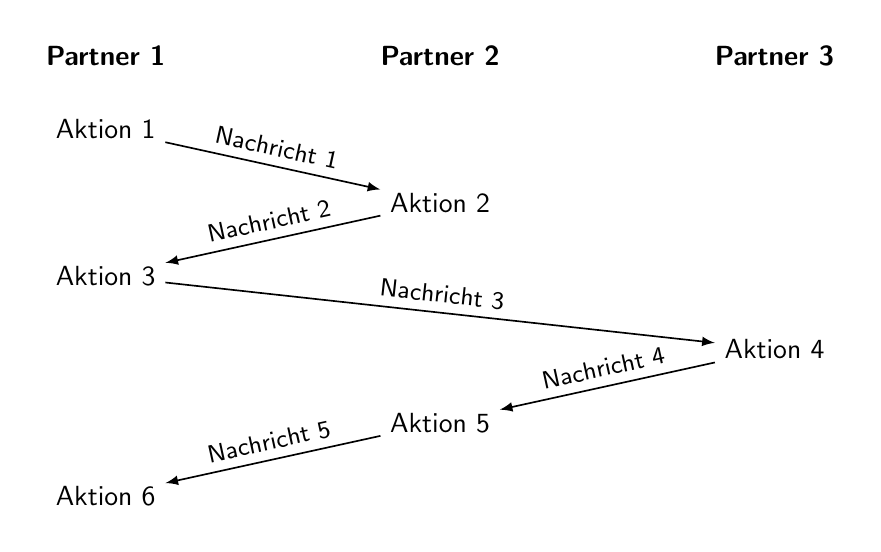
\begin{tikzpicture}[
every node/.append style={font={\sffamily}},
caption/.append style={font={\sffamily\bfseries}},
comm/.style={-latex,semithick},
msg/.style={midway,sloped,above,font={\sffamily\small}},
]
\matrix[row sep=3ex,column sep=25mm] {
\node[caption] {Partner 1};  & \node[caption] {Partner 2}; & \node[caption] {Partner 3}; \\
\node (A1) {Aktion 1}; & & \\
& \node (A2) {Aktion 2}; & \\
\node (A3) {Aktion 3}; & & \\
& & \node (A4) {Aktion 4};\\
& \node (A5) {Aktion 5}; & \\
\node (A6) {Aktion 6}; & & \\
};

\draw[comm] (A1)--(A2) node[msg] {Nachricht 1};
\draw[comm] (A2)--(A3) node[msg] {Nachricht 2};
\draw[comm] (A3)--(A4) node[msg] {Nachricht 3};
\draw[comm] (A4)--(A5) node[msg] {Nachricht 4};
\draw[comm] (A5)--(A6) node[msg] {Nachricht 5};

\end{tikzpicture}%
	}%
	\caption{Netzwerkkommunikationsgraph mit TikZ}%
  \label{fig:net-comm}%
\end{figure}

\begin{figure}[hp]%
	\centering%
	\subfloat[Ursprünglicher Merkmalsraum]{%
		\label{fig:ica-1}%
		\tikzsetnextfilename{ica-1}%
		\resizebox{0.45\textwidth}{!}{%
			\begin{tikzpicture}[
my_plot/.style={draw=none,every mark/.append style={draw=KITblue,fill=KITblue},mark=*,mark size=1.5pt},
]

\begin{axis}[
width=4cm,
height=4cm,
xmin = -1.1,
xmax = 1.1,
xlabel={$m_1$},
ymin = -1.1,
ymax = 1.1,
ylabel={$m_2$},
axis lines=center,
scale only axis,
]

\addplot[my_plot] coordinates {
(0.030,-0.062) (-0.118,-0.004) (0.276,0.236) (0.578,0.566) (-0.143,-0.014)
(0.304,0.257) (0.423,0.535) (0.205,0.344) (0.364,0.365) (-0.327,-0.368)
(0.176,0.310) (-0.298,-0.360) (0.153,0.279) (0.010,0.062) (0.150,0.231)
(-0.301,-0.214) (0.079,0.094) (-0.241,-0.161) (-0.474,-0.461) (0.091,0.173)
(0.541,0.601) (-0.288,-0.153) (0.013,-0.093) (0.290,0.115) (0.194,0.028)
(0.486,0.370) (0.201,0.227) (0.510,0.510) (-0.211,-0.293) (-0.058,0.088)
(0.326,0.176) (-0.591,-0.574) (0.071,0.204) (-0.401,-0.308) (0.206,0.111)
(-0.529,-0.667) (0.064,0.040) (0.032,0.035) (-0.349,-0.291) (0.476,0.316)
(0.625,0.624) (0.312,0.234) (0.076,-0.079) (0.016,0.018) (-0.556,-0.655)
(-0.308,-0.217) (0.248,0.122) (-0.515,-0.428) (-0.121,0.041) (0.260,0.228)
(-0.317,-0.406) (0.650,0.483) (-0.198,-0.097) (-0.427,-0.495) (0.429,0.553)
(-0.432,-0.538) (-0.460,-0.440) (-0.558,-0.654) (0.516,0.586) (-0.230,-0.205)
(0.148,0.199) (-0.417,-0.240) (-0.138,-0.040) (-0.252,-0.403) (0.096,0.010)
(-0.478,-0.339) (0.628,0.650) (0.054,-0.104) (0.502,0.429) (0.051,0.045)
(0.099,0.106) (0.344,0.214) (-0.359,-0.334) (0.291,0.187) (0.176,0.217)
(0.329,0.362) (-0.270,-0.116) (-0.136,-0.008) (-0.446,-0.533) (0.653,0.585)
(0.474,0.540) (0.093,0.136) (0.356,0.473) (0.232,0.217) (0.592,0.659)
(-0.326,-0.170) (-0.683,-0.497) (-0.484,-0.357) (-0.607,-0.635) (-0.044,-0.041)
(-0.681,-0.533) (-0.306,-0.401) (0.189,0.334) (0.420,0.259) (0.040,0.086)
(-0.148,-0.303) (-0.585,-0.507) (0.424,0.330) (0.597,0.688) (0.211,0.271)
(-0.429,-0.360) (0.280,0.188) (0.375,0.252) (-0.505,-0.528) (-0.064,-0.043)
(-0.257,-0.140) (0.302,0.262) (-0.228,-0.293) (0.154,0.122) (-0.549,-0.403)
(0.034,-0.027) (0.207,0.122) (-0.538,-0.648) (-0.601,-0.664) (-0.623,-0.433)
(-0.552,-0.417) (-0.094,-0.166) (0.469,0.496) (0.580,0.497) (0.212,0.159)
(0.515,0.627) (-0.070,-0.167) (-0.101,-0.015) (-0.244,-0.328) (-0.372,-0.477)
(0.256,0.199) (-0.607,-0.560) (-0.462,-0.554) (0.132,0.086) (0.066,0.050)
(0.230,0.157) (-0.502,-0.556) (0.666,0.490) (0.407,0.425) (-0.219,-0.355)
(-0.250,-0.285) (0.266,0.159) (-0.263,-0.412) (0.028,0.091) (-0.086,0.043)
(-0.633,-0.504) (-0.420,-0.399) (0.378,0.380) (-0.008,-0.163) (-0.226,-0.278)
(0.148,0.193) (-0.629,-0.582) (0.586,0.450) (0.025,0.136) (-0.445,-0.360)
};

\end{axis}
\end{tikzpicture}
		}%
	}%
	\hfill%
	\subfloat[Transienter Merkmalsraum (Nach Whitening, z.\,B. durch \gls{ac:PCA} inkl. Normalisierung)]{%
		\label{fig:ica-2}%
		\tikzsetnextfilename{ica-2}%
		\resizebox{0.45\textwidth}{!}{%
			\begin{tikzpicture}[
my_plot/.style={draw=none,every mark/.append style={draw=KITblue,fill=KITblue},mark=*,mark size=1.5pt},
]

\begin{axis}[
width=4cm,
height=4cm,
xmin = -1.1,
xmax = 1.1,
xlabel={$m'_1$},
ymin = -1.1,
ymax = 1.1,
ylabel={$m'_2$},
axis lines=center,
scale only axis,
]

\addplot[my_plot] coordinates {
(-0.273,-0.278) (0.267,0.398) (0.117,-0.289) (0.483,-0.399) (0.293,0.455)
(0.120,-0.326) (0.747,0.049) (0.640,0.265) (0.329,-0.231) (-0.430,0.090)
(0.597,0.269) (-0.471,0.014) (0.549,0.259) (0.180,0.141) (0.401,0.136)
(0.014,0.439) (0.120,-0.008) (0.044,0.379) (-0.384,0.338) (0.349,0.173)
(0.681,-0.175) (0.183,0.566) (-0.335,-0.309) (-0.310,-0.678) (-0.368,-0.593)
(0.057,-0.637) (0.266,-0.054) (0.457,-0.325) (-0.457,-0.098) (0.425,0.450)
(-0.196,-0.631) (-0.474,0.426) (0.500,0.334) (-0.059,0.516) (-0.127,-0.402)
(-0.926,-0.054) (-0.019,-0.107) (0.038,-0.012) (-0.122,0.388) (-0.094,-0.754)
(0.560,-0.398) (0.026,-0.418) (-0.439,-0.488) (0.021,-0.004) (-0.822,0.075)
(0.020,0.454) (-0.190,-0.516) (-0.180,0.573) (0.420,0.535) (0.130,-0.255)
(-0.575,-0.050) (0.039,-0.885) (0.151,0.410) (-0.607,0.078) (0.790,0.077)
(-0.736,-0.026) (-0.348,0.349) (-0.817,0.082) (0.692,-0.130) (-0.126,0.216)
(0.301,0.052) (0.202,0.765) (0.195,0.363) (-0.719,-0.267) (-0.195,-0.306)
(0.024,0.696) (0.635,-0.338) (-0.469,-0.483) (0.215,-0.523) (0.028,-0.048)
(0.113,-0.042) (-0.116,-0.587) (-0.242,0.298) (-0.078,-0.479) (0.291,0.003)
(0.405,-0.114) (0.259,0.605) (0.297,0.450) (-0.684,0.038) (0.365,-0.607)
(0.644,-0.112) (0.223,0.062) (0.701,0.104) (0.158,-0.192) (0.752,-0.185)
(0.214,0.646) (-0.007,0.960) (-0.020,0.667) (-0.635,0.308) (-0.029,0.037)
(-0.131,0.849) (-0.587,-0.076) (0.645,0.292) (-0.150,-0.724) (0.184,0.102)
(-0.638,-0.344) (-0.270,0.594) (0.073,-0.536) (0.833,-0.122) (0.385,0.036)
(-0.160,0.468) (-0.048,-0.437) (-0.065,-0.586) (-0.531,0.254) (0.010,0.099)
(0.151,0.495) (0.141,-0.305) (-0.417,-0.039) (0.033,-0.188) (-0.016,0.763)
(-0.166,-0.191) (-0.093,-0.373) (-0.843,0.031) (-0.746,0.204) (0.060,0.933)
(-0.055,0.733) (-0.320,-0.144) (0.510,-0.221) (0.252,-0.601) (0.018,-0.283)
(0.829,-0.011) (-0.381,-0.230) (0.190,0.308) (-0.492,-0.081) (-0.679,-0.062)
(0.042,-0.326) (-0.391,0.520) (-0.717,0.032) (-0.032,-0.214) (0.009,-0.085)
(-0.034,-0.355) (-0.627,0.168) (0.022,-0.923) (0.424,-0.209) (-0.641,-0.245)
(-0.339,0.060) (-0.110,-0.472) (-0.722,-0.253) (0.230,0.160) (0.345,0.421)
(-0.147,0.768) (-0.309,0.326) (0.348,-0.233) (-0.513,-0.434) (-0.372,-0.002)
(0.278,0.031) (-0.413,0.531) (0.082,-0.757) (0.384,0.297) (-0.122,0.523)
};

\end{axis}
\end{tikzpicture}%
		}%
	}%
	\hfill%
	\subfloat[Transformierter Merkmalsraum]{%
		\label{fig:ica-3}%
		\tikzsetnextfilename{ica-3}%
		\resizebox{0.45\textwidth}{!}{%
			\begin{tikzpicture}[
my_plot/.style={draw=none,every mark/.append style={draw=KITblue,fill=KITblue},mark=*,mark size=1.5pt},
]

\begin{axis}[
width=4cm,
height=4cm,
xmin = -1.1,
xmax = 1.1,
xlabel={$m''_1$},
ymin = -1.1,
ymax = 1.1,
ylabel={$m''_2$},
axis lines=center,
scale only axis,
]

\addplot[my_plot] coordinates {
(-0.389,-0.004) (0.470,0.093) (-0.122,-0.287) (0.059,-0.623) (0.529,0.115)
(-0.146,-0.316) (0.563,-0.493) (0.640,-0.265) (0.069,-0.396) (-0.241,0.367)
(0.613,-0.232) (-0.323,0.342) (0.572,-0.205) (0.227,-0.027) (0.379,-0.188)
(0.320,0.300) (0.079,-0.090) (0.299,0.237) (-0.033,0.510) (0.369,-0.124)
(0.358,-0.605) (0.530,0.271) (-0.455,0.019) (-0.699,-0.260) (-0.680,-0.159)
(-0.410,-0.491) (0.150,-0.226) (0.093,-0.554) (-0.393,0.254) (0.619,0.017)
(-0.584,-0.307) (-0.034,0.636) (0.590,-0.118) (0.323,0.406) (-0.374,-0.194)
(-0.693,0.617) (-0.089,-0.062) (0.018,-0.035) (0.188,0.361) (-0.600,-0.467)
(0.114,-0.678) (-0.277,-0.314) (-0.655,-0.035) (0.012,-0.018) (-0.528,0.634)
(0.335,0.306) (-0.499,-0.230) (0.278,0.532) (0.676,0.081) (-0.088,-0.272)
(-0.442,0.371) (-0.599,-0.654) (0.397,0.183) (-0.374,0.484) (0.613,-0.504)
(-0.539,0.502) (0.001,0.493) (-0.520,0.635) (0.398,-0.581) (0.063,0.242)
(0.249,-0.176) (0.684,0.398) (0.395,0.119) (-0.697,0.320) (-0.354,-0.078)
(0.509,0.475) (0.210,-0.688) (-0.674,-0.010) (-0.218,-0.522) (-0.014,-0.053)
(0.050,-0.110) (-0.498,-0.333) (0.040,0.382) (-0.394,-0.284) (0.208,-0.204)
(0.206,-0.367) (0.611,0.245) (0.528,0.108) (-0.457,0.510) (-0.171,-0.688)
(0.376,-0.535) (0.202,-0.114) (0.569,-0.422) (-0.024,-0.247) (0.401,-0.663)
(0.608,0.305) (0.674,0.684) (0.457,0.486) (-0.231,0.667) (0.005,0.047)
(0.508,0.693) (-0.469,0.362) (0.663,-0.250) (-0.618,-0.406) (0.203,-0.058)
(-0.694,0.208) (0.229,0.611) (-0.327,-0.431) (0.503,-0.676) (0.298,-0.247)
(0.217,0.444) (-0.343,-0.275) (-0.460,-0.368) (-0.196,0.555) (0.077,0.063)
(0.457,0.243) (-0.116,-0.315) (-0.322,0.267) (-0.110,-0.157) (0.528,0.550)
(-0.253,-0.018) (-0.329,-0.198) (-0.574,0.618) (-0.384,0.672) (0.702,0.617)
(0.480,0.557) (-0.329,0.124) (0.205,-0.517) (-0.247,-0.604) (-0.188,-0.213)
(0.578,-0.594) (-0.432,0.106) (0.352,0.083) (-0.406,0.291) (-0.523,0.436)
(-0.201,-0.260) (0.091,0.644) (-0.484,0.530) (-0.173,-0.129) (-0.054,-0.067)
(-0.275,-0.227) (-0.325,0.562) (-0.637,-0.668) (0.152,-0.447) (-0.626,0.280)
(-0.197,0.283) (-0.411,-0.256) (-0.690,0.332) (0.276,-0.050) (0.542,0.054)
(0.439,0.647) (0.012,0.449) (0.081,-0.411) (-0.670,0.056) (-0.265,0.262)
(0.218,-0.175) (0.083,0.668) (-0.477,-0.594) (0.482,-0.061) (0.284,0.456)
};

\end{axis}
\end{tikzpicture}%
		}%
}%
\caption{Diagramme mit TikZ direkt in LaTeX (hier: Die Schritte der \enquote{Independent component analysis})}%
\label{fig:ica}%
\end{figure}

\begin{figure}[hp]
	\centering%
	\subfloat[Ungünstige Projektion]{%
		\label{fig:pca-1}%
		\tikzsetnextfilename{pca-1}%
		\resizebox{0.48\textwidth}{!}{%
			\begin{tikzpicture}[
my_plot_1/.style={draw=none,every mark/.append style={draw=KITblue,fill=KITblue},mark=*},
my_plot_2/.style={draw=none,every mark/.append style={draw=KITred,fill=KITred},mark=*},
trans_arrow/.style={semithick,KITorange,-latex},
]

\begin{axis}[
width=4cm,
height=4cm,
xmin = -0.2,
xmax = 2.3,
xlabel={$m_1$},
ymin = -0.2,
ymax = 2.3,
ylabel={$m_2$},
xticklabel=\empty,
yticklabel=\empty,
axis lines=center,
clip=false,
scale only axis,
]

\addplot[my_plot_1] coordinates {
(1.3,0.38)
(1.42,0.71)
(1.48,0.60)
(1.64,0.54)
(1.65,0.81)
(1.68,0.89)
(1.79,1.11)
(1.88,1.18)
(1.89,1.46)
(1.94,1.35)
(1.86,1.65)
(2.02,1.83)
(2.12,1.83)
(2.19,2.26)
(2.21,2.07)
};

\addplot[my_plot_2] coordinates {
(1.28,0.58)
(1.33,0.93)
(1.54,1.03)
(1.54,1.26)
(1.51,1.41)
(1.72,1.52)
(1.76,1.87)
(1.80,1.90)
(1.90,2.00)
(1.91,2.27)
(2.05,2.40)
};

\coordinate(CoM) at (axis cs:1.71,1.38) {};

\draw[trans_arrow] (axis cs:0,0)--(CoM) node[midway,above left] {$m_0$};

\end{axis}

\begin{axis}[
width=5cm,
height=2.5cm,
xmin = -1.5,
xmax = 1.5,
xlabel={$m'_1$},
ymin = -0.75,
ymax = 0.75,
ylabel={$m'_2$},
axis lines=center,
xlabel style={anchor=north west},
ylabel style={anchor=south west},
xticklabel=\empty,
yticklabel=\empty,
clip=false,
anchor=origin,
at={(CoM)},
rotate around={65:(current axis.origin)},
clip=false,
scale only axis
]

\addplot+[my_plot_1] coordinates {
(-2,-0.0510)
(-2,-0.0203)
(-2,-0.1212)
(-2,-0.2916)
(-2,-0.1865)
(-2,-0.1799)
(-2,-0.1866)
(-2,-0.2386)
(-2,-0.1293)
(-2,-0.2211)
(-2,-0.0218)
(-2,-0.0908)
(-2,-0.1814)
(-2,-0.0631)
(-2,-0.1615)
};

\addplot+[my_plot_2] coordinates {
(-2,0.0516)
(-2,0.1542)
(-2,0.0062)
(-2,0.1034)
(-2,0.1939)
(-2,0.0501)
(-2,0.1618)
(-2,0.1382)
(-2,0.0898)
(-2,0.1949)
(-2,0.1229)
};

\draw[trans_arrow,shorten <=2pt,shorten >=3pt] (axis cs:-1.5,0)--(axis cs:-2,0) node[midway,right,font={\footnotesize},align=left] {Projektion\\auf $e_2$};
\draw[semithick] (axis cs:-2,-0.5)--(axis cs:-2,0.4);

\addplot+[my_plot_1] coordinates {
(-1.0796,-1.5)
(-0.7298,-1.5)
(-0.8041,-1.5)
(-0.7909,-1.5)
(-0.5420,-1.5)
(-0.4568,-1.5)
(-0.2109,-1.5)
(-0.1094,-1.5)
(0.1486,-1.5)
(0.0700,-1.5)
(0.3081,-1.5)
(0.5389,-1.5)
(0.5811,-1.5)
(1.0004,-1.5)
(0.8367,-1.5)
};

\addplot+[my_plot_2] coordinates {
(-0.9068,-1.5)
(-0.5684,-1.5)
(-0.3891,-1.5)
(-0.1806,-1.5)
(-0.0573,-1.5)
(0.1311,-1.5)
(0.4652,-1.5)
(0.5093,-1.5)
(0.6422,-1.5)
(0.8911,-1.5)
(1.0681,-1.5)
};

\draw[trans_arrow,shorten <=2pt,shorten >=3pt] (axis cs:0,-0.75)--(axis cs:0,-1.5) node[midway,anchor=north east,font={\footnotesize},align=left] {Projektion\\auf $e_1$};
\draw[semithick] (axis cs:-1.3,-1.5)--(axis cs:1.3,-1.5);

\end{axis}

\end{tikzpicture}%
		}%
	}\hfill%
	\subfloat[Zielführende Projektion]{%
		\label{fig:pca-2}%
		\tikzsetnextfilename{pca-2}%
		\resizebox{0.48\textwidth}{!}{%
			\begin{tikzpicture}[
my_plot_1/.style={draw=none,every mark/.append style={draw=KITblue,fill=KITblue},mark=*},
my_plot_2/.style={draw=none,every mark/.append style={draw=KITred,fill=KITred},mark=*},
trans_arrow/.style={semithick,KITorange,-latex},
]

\begin{axis}[
width=4cm,
height=4cm,
xmin = -0.2,
xmax = 2.3,
xlabel={$m_1$},
ymin = -0.2,
ymax = 2.3,
ylabel={$m_2$},
xticklabel=\empty,
yticklabel=\empty,
axis lines=center,
clip=false,
scale only axis,
]

\addplot[my_plot_1] coordinates {
(1.3,0.38)
(1.28,0.58)
(1.42,0.71)
(1.48,0.60)
(1.64,0.54)
(1.33,0.93)
(1.65,0.81)
(1.68,0.89)
(1.54,1.03)
(1.54,1.26)
(1.79,1.11)
(1.88,1.18)
(1.51,1.41)
};

\addplot[my_plot_2] coordinates {
(1.72,1.52)
(1.89,1.46)
(1.94,1.35)
(1.86,1.65)
(1.76,1.87)
(1.80,1.90)
(1.90,2.00)
(2.02,1.83)
(2.12,1.83)
(1.91,2.27)
(2.19,2.26)
(2.21,2.07)
(2.05,2.40)
};

\coordinate(CoM) at (axis cs:1.71,1.38) {};

\draw[trans_arrow] (axis cs:0,0)--(CoM) node[midway,above left] {$m_0$};

\end{axis}

\begin{axis}[
width=5cm,
height=2.5cm,
xmin = -1.5,
xmax = 1.5,
xlabel={$m'_1$},
ymin = -0.75,
ymax = 0.75,
ylabel={$m'_2$},
axis lines=center,
xlabel style={anchor=north west},
ylabel style={anchor=south west},
xticklabel=\empty,
yticklabel=\empty,
clip=false,
anchor=origin,
at={(CoM)},
rotate around={65:(current axis.origin)},
clip=false,
scale only axis
]

\addplot+[my_plot_1] coordinates {
(-2,-0.0510)
(-2,0.0516)
(-2,-0.0203)
(-2,-0.1212)
(-2,-0.2916)
(-2,0.1542)
(-2,-0.1865)
(-2,-0.1799)
(-2,0.0062)
(-2,0.1034)
(-2,-0.1866)
(-2,-0.2386)
(-2,0.1939)
};

\addplot+[my_plot_2] coordinates {
(-2,0.0501)
(-2,-0.1293)
(-2,-0.2211)
(-2,-0.0218)
(-2,0.1618)
(-2,0.1382)
(-2,0.0898)
(-2,-0.0908)
(-2,-0.1814)
(-2,0.1949)
(-2,-0.0631)
(-2,-0.1615)
(-2,0.1229)
};

\draw[trans_arrow,shorten <=2pt,shorten >=3pt] (axis cs:-1.5,0)--(axis cs:-2,0) node[midway,right,font={\footnotesize},align=left] {Projektion\\auf $e_2$};
\draw[semithick] (axis cs:-2,-0.5)--(axis cs:-2,0.4);

\addplot+[my_plot_1] coordinates {
(-1.0796,-1.5)
(-0.9068,-1.5)
(-0.7298,-1.5)
(-0.8041,-1.5)
(-0.7909,-1.5)
(-0.5684,-1.5)
(-0.5420,-1.5)
(-0.4568,-1.5)
(-0.3891,-1.5)
(-0.1806,-1.5)
(-0.2109,-1.5)
(-0.1094,-1.5)
(-0.0573,-1.5)
};

\addplot+[my_plot_2] coordinates {
(0.1311,-1.5)
(0.1486,-1.5)
(0.0700,-1.5)
(0.3081,-1.5)
(0.4652,-1.5)
(0.5093,-1.5)
(0.6422,-1.5)
(0.5389,-1.5)
(0.5811,-1.5)
(0.8911,-1.5)
(1.0004,-1.5)
(0.8367,-1.5)
(1.0681,-1.5)
};

\draw[trans_arrow,shorten <=2pt,shorten >=3pt] (axis cs:0,-0.75)--(axis cs:0,-1.5) node[midway,anchor=north east,font={\footnotesize},align=left] {Projektion\\auf $e_1$};
\draw[semithick] (axis cs:-1.3,-1.5)--(axis cs:1.3,-1.5);

\end{axis}

\end{tikzpicture}%
		}%
	}%
	\caption{Aufwändiges Diagramm mit TikZ (hier: Probleme der \enquote{Principal component analysis})}%
	\label{fig:pca}%
\end{figure}